\chapter{Конструкторская часть}

В данном разделе представлены схема алгоритма поиска строчной координаты элементы матрицы РСФ.

\section{Требования к программному обеспечению}

К программе предъявлены ряд требований:

\begin{itemize}[label=---]
	\item наличие интерфейса для ввода матрицы и индекс искомого элемента;
	\item вывод матрицы в виде РСФ после ввода, то есть трех массивов;
	\item вывод пошагового работы алгоритма поиска строчной координаты элемента матрицы.
\end{itemize}

\section{Разработка алгоритмов}

На рисунке~\ref{fig:csr_diag} представлен алгоритма поиска строчной координаты элементы матрицы РСФ.

\begin{figure}[h]
	\centering
	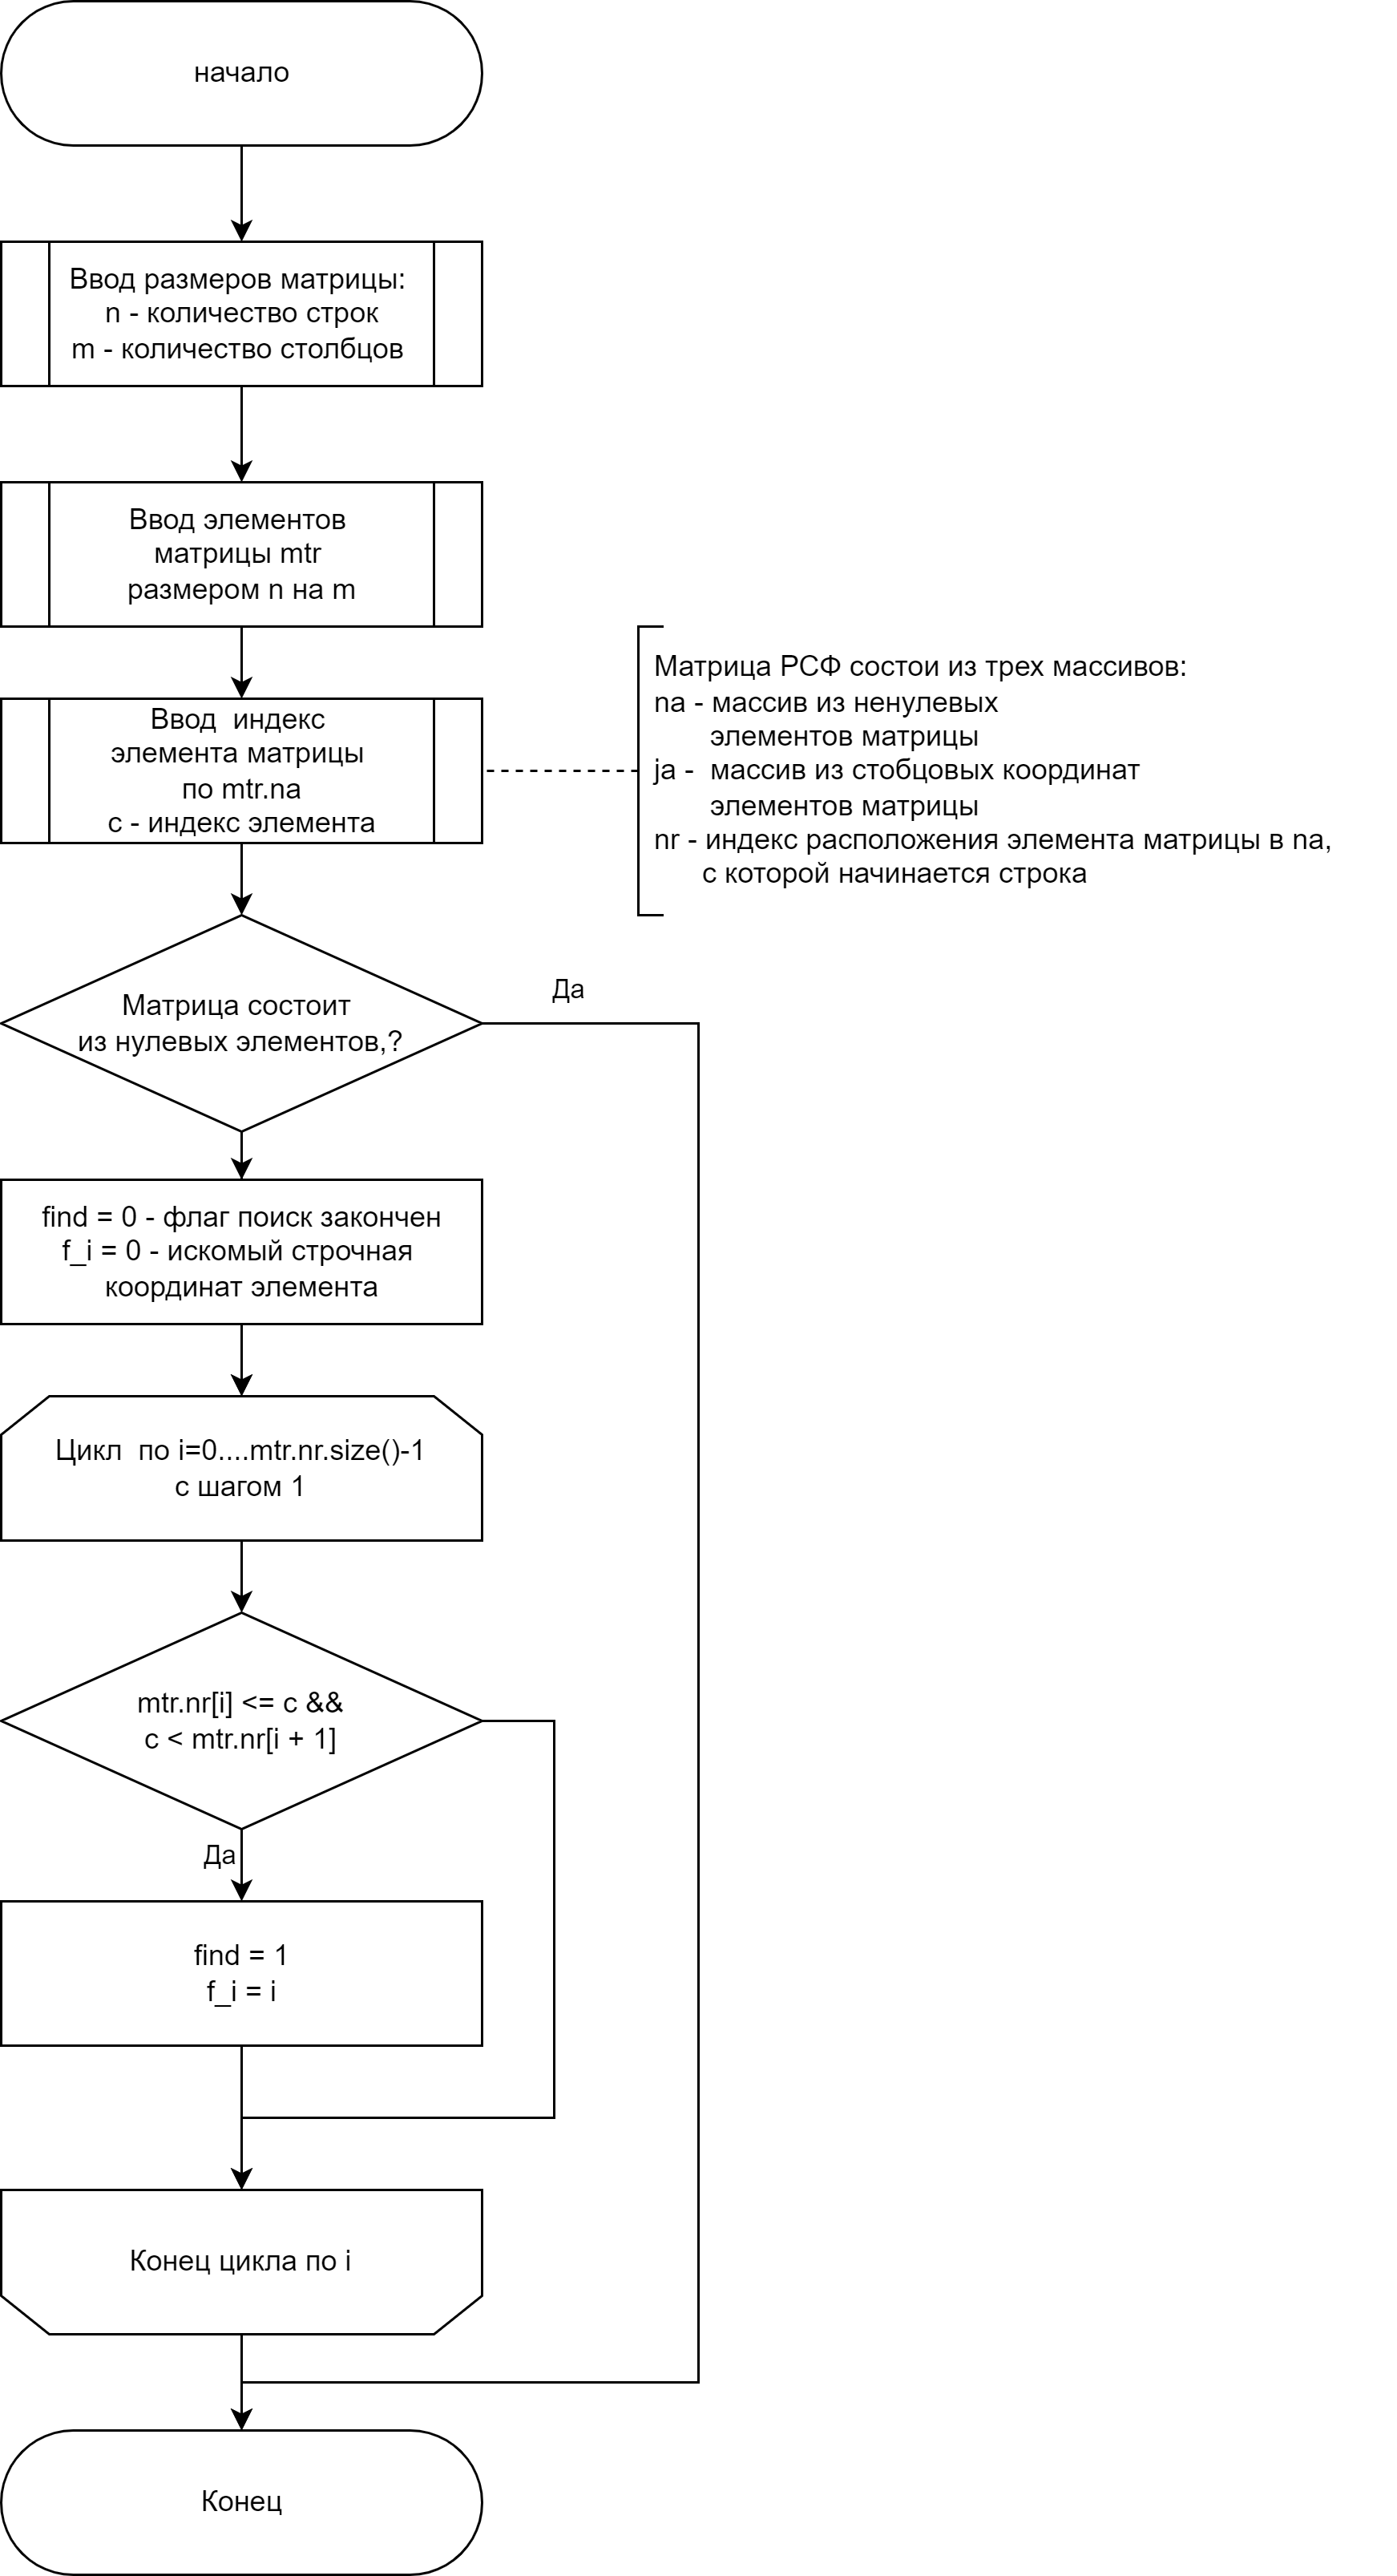
\includegraphics[height=0.85\textheight]{img/alg.png}
	\caption{Схема алгоритма поиска строчной координаты элементы матрицы РСФ}
	\label{fig:csr_diag}
\end{figure}

\clearpage

\section*{Вывод}
В данном разделе представлена схема алгоритма поиска строчной координаты матрицы РСФ и выдвинуты требования к программному обеспечению.